
%(BEGIN_QUESTION)
% Copyright 2007, Tony R. Kuphaldt, released under the Creative Commons Attribution License (v 1.0)
% This means you may do almost anything with this work of mine, so long as you give me proper credit

Examine this process trend, showing the response of the process variable to a 10\% up-and-down step change in the controller output (placed in manual mode):

$$\includegraphics[width=15.5cm]{i01721x01.eps}$$

What characteristics of the process (and its related instrumentation) can you discern from this trend?  Based on this information, do you think the process might benefit from a controller with aggressive P, I, or D action?  Explain why or why not for each action.

\vskip 10pt

Suppose a fellow instrument technician looked over your shoulder at this trend graph and declared, ``I see a lot of integral action in that controller!''  What would you say to that comment?  Is it helpful in determining how the controller {\it ought} to be tuned?  Explain why or why not.

\vskip 20pt \vbox{\hrule \hbox{\strut \vrule{} {\bf Suggestions for Socratic discussion} \vrule} \hrule}

\begin{itemize}
\item{} One area of confusion for new students is whether any given trend graph reveals an {\it open-loop} test or a {\it closed-loop} test.  Explain how it is possible to discern the kind of test done on this process just by looking at the trend lines.
\item{} Explain why it is important to determine whether the trend graph reveals an {\it open-loop} test or a {\it closed-loop} test.  What difference does this determination make?
\item{} What type of physical process (e.g. gas pressure, liquid temperature, gas flow, etc.) do you think this might be, based solely on the trend you see here?
\item{} Based on what you see here, does the controller need to be configured for {\it direct} action or for {\it reverse} action?
\end{itemize}

\underbar{file i01721}
%(END_QUESTION)





%(BEGIN_ANSWER)

This is an {\it integrating} process, and as such it should respond well to aggressive proportional action.  

\vskip 10pt

The ramping we see in the PV following the output step-change tells us absolutely nothing about the status of the controller, but rather how the process itself happens to react to changes in its stimulus (the FCE).  The mistake of interpreting open-loop (manual mode) tests as indicators of controller action is based on the person not noticing or appreciating the fact that the controller is in manual mode.  In manual mode, the response we see in the PV following the output signal change is due entirely to the physics of the process, not the programming of the controller.

%(END_ANSWER)





%(BEGIN_NOTES)

The integrating nature of this process is revealed by two traits: the roughly constant slope (linear shape) of the process response following the output step-change, and also the fact that the process variable levels off and stabilizes at a new value when the output returns to its former value.

In a case like this, I would suggest increasing the controller gain up as far as practical while maintaining loop stability, then adding just enough integral action to overcome the inevitable proportional-only offset.

%INDEX% Control, PID tuning: predicting PID requirements based on open-loop response

%(END_NOTES)


